\documentclass [xcolor=svgnames, t] {beamer} 
\usepackage[utf8]{inputenc}
\usepackage{booktabs, comment} 
\usepackage[absolute, overlay]{textpos} 
\usepackage{pgfpages}
\usepackage[font=footnotesize]{caption}
\useoutertheme{infolines} 



%\definecolor{brownbrown}{RGB}{56, 28, 0}
%\definecolor{brownred}{RGB}{228, 0, 43}

%\setbeamercolor{title in head/foot}{bg=brownred, fg=brownbrown}
%\setbeamercolor{author in head/foot}{bg=myuniversity}
\setbeamertemplate{page number in head/foot}{}
\usepackage{csquotes}


\usepackage{amsmath}
\usepackage[makeroom]{cancel}


\usepackage{textpos}

\usepackage{tikz}

\usetheme{Madrid}
%\definecolor{myuniversity}{RGB}{56, 28, 0}
%\usecolortheme[named=myuniversity]{structure}
\usepackage{tikz}



\title[Introducci\'on]{Clase No.0: Introducci\'on}
\subtitle{Objetivos, metodolog\'ia y evaluaci\'on}
\institute[]{Departamento de Ingenier\'ia Civil y Agr\'icola\\ Facultad de Ingenier\'ia  \\Universidad Nacional de Colombia - Sede Bogot\'a}
\titlegraphic{
\includegraphics[height=2.0cm]{escudoUnal.png}}
\author[LAM]{Luis Alejandro Morales \\ \href{https://lamhydro.github.io}{https://lamhydro.github.io}}


%\institute[]{Department of Earth, Environmental, and Planetary Sciences  \\Brown University}
\date{\today}


\addtobeamertemplate{navigation symbols}{}{%
    \usebeamerfont{footline}%
    \usebeamercolor[fg]{footline}%
    \hspace{1em}%
    \insertframenumber/\inserttotalframenumber
}

\begin{document}
\begin{frame}
\maketitle
\end{frame}


%%%%%%%%%%%%%%%%%%%%%%%%%%%%
\logo{\vspace{-0.2cm}
\includegraphics[height=0.8cm]{escudoUnal.png}~%
}
%%%%%%%%%%%%%%%%%%%%%%%%%%



\begin{frame}
\frametitle{Table of Contents}
\tableofcontents
\end{frame}

%\section{Acerca de mi}
%\begin{frame}{Estudios}
%\begin{itemize}
%\item Pregrado: \textbf{Ingenier\'ia Civil}, \emph{Escuela Colombiana de Ingenier\'ia} - (2002)
%\item Especializaci\'on: \textbf{Recursos Hidr\'aulicos y Medio Ambiente}, \emph{Escuela Colombiana de Ingenier\'ia} - (2003)
%\item Maestria: \textbf{Ingenier\'ia de Recursos Hidr\'aulicos}, \emph{Universidad Nacional de Colombia - Sede Bogot\'a} - (2007)
%\item Ph.D.: \textbf{Geograf\'ia F\'isica (Major Hidrolog\'ia)}, \emph{University College London (UCL)} - (2013)
%\end{itemize}
%\end{frame}
%
%
%\begin{frame}{Experiencia}
%\begin{itemize}
%\item Teaching: \textbf{Programaci\'on en UNIX/Linux}, \emph{University College London (UCL)} - (2008-2013)
%\item Teaching: \textbf{River Science}, \emph{Global Institute for Water Security (GIWS)-University of Saskatchewan} - (2013-2019)
%\item Postdoctoral Reseach Fellow: \textbf{Modelaci\'on hidrol\'ogica y de calidad de agua}, \emph{Global Institute for Water Security (GIWS)-University of Saskatchewan} - (2013-2019)
%\item Physical Scientist: \textbf{Modelaci\'on y predicci\'on hidrol\'ogica}, \emph{Environment and Climate Change Canada (ECCC) - Gobernment of Canada} - (2019-2022)
%\end{itemize}
%\end{frame}
%
%\begin{frame}{Mis sitios}
%\begin{block}{Website}
%\href{https://lamhydro.github.io}{https://lamhydro.github.io}
%\end{block}
%
%\begin{block}{Otros}
%\begin{itemize}
%\item \href{https://scholar.google.ca/citations?user=Lc95RL0AAAAJ&hl=en}{Google Scholar}
%\item \href{https://www.researchgate.net/profile/Luis-Morales-Marin}{Research Gate}
%\end{itemize}
%\end{block}
%\end{frame}

\section{Generalidades}
\begin{frame}{Informaci\'on}
\begin{exampleblock}{}
\begin{itemize}
\item \alert{Oficina}: Edificio Laboratorio de Hidr\'aulica (409), oficina 305 
\item \alert{Email}: lmoralesm@unal.edu.co
\end{itemize}
\end{exampleblock}
\end{frame}

\begin{frame}{La asignatura}
\begin{itemize}
\item Identificaci\'on de la asignatura: \alert{2015966}
\item Duraci\'on clase presencial: \alert{5 hrs/semana}
\item No. de semanas: \alert{16}
\item No. de cr\'editos: \alert{4}
\item ¿Esta asignatura es validable?: \alert{No}
\item ¿Asignatura de libre elecci\'on?: \alert{No}
\item Planes de estudio a los que se asocia la asignatura
\begin{itemize}
\item \alert{2540 Ingenier\'ia Agr\'icola Componente C}
\item \alert{2541 Ingenier\'ia Civil Componente C}
\end{itemize}
\item Prerequisitos
\begin{itemize}
\item \alert{C\'alculo en varias variables}
\item \alert{Ecuaciones diferenciales}
\item \alert{Est\'atica}
\end{itemize}
\end{itemize}
\end{frame}

\begin{frame}{P\'agina de la asignatura}
\begin{block}{P\'agina de la asignatura}
\href{https://lamhydro.github.io/fluidMechanics/}{https://lamhydro.github.io/fluidMechanics/}
\end{block}
\end{frame}

\section{Horario de clases}
\begin{frame}{Horario de clases}
\centering
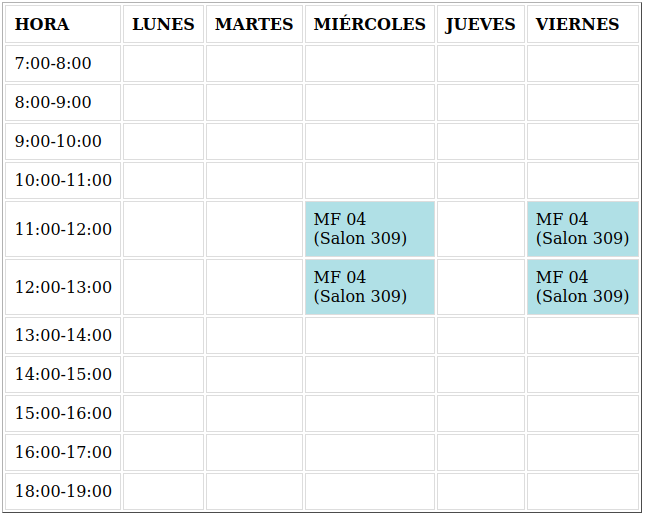
\includegraphics[width=9cm]{horarioClases}
\end{frame}

\section{Descripci\'on}
\begin{frame}{Descripci\'on}
\vspace{-0.8cm} 
\begin{columns}
\column{0.6\textwidth}
\begin{exampleblock}{}
\small
La asignatura mecánica de fluidos se centra en el estudio y análisis de las propiedades físicas más relevantes de los fluidos a partir de los aspectos fundamentales de la física, el cálculo y las ecuaciones diferenciales. Con ello el curso se centra en el estudio y aplicación de \alert{cuatro principios: de Pascal, de conservación de la masa, de conservación de la energía, momentum lineal y angular}, principios que se aplican a diferentes condiciones de contorno a los cuales están sometidos los fluidos. Finalmente se hace una introducción al análisis dimensional y semejanza hidráulica.
\end{exampleblock}
\column{0.4\textwidth}
\begin{center}
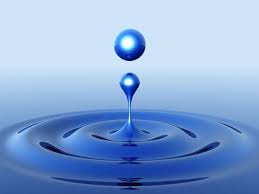
\includegraphics[width=\textwidth]{fm}
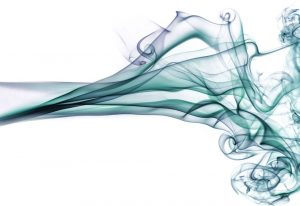
\includegraphics[width=\textwidth]{fm1}
\end{center}
\end{columns}
\end{frame}


\section{Conceptos previos necesarios}
\begin{frame}{Conceptos previos necesarios}
\begin{exampleblock}{}
El curso requiere el uso de herramientas matemáticas para la solución de \alert{ecuaciones diferenciales} y el entendimiento básico de los teoremas fundamentales del \alert{cálculo multivariado}, así como los conocimientos básicos de Estática. Es deseable que los estudiantes tengan conocimientos básicos en programación de computadores y el manejo de herramientas de métodos numéricos.
\end{exampleblock}
\end{frame}

\section{Objetivo}
\begin{frame}{Objetivo}
\begin{columns}
\column{0.6\textwidth}
\begin{exampleblock}{}
Dar a conocer las \alert{leyes físicas fundamentales} que tienen que ver con el comportamiento de los fluidos y sus aplicaciones a \alert{problemas típicos de la Ingeniería}. Al finalizar el curso, el estudiante debe estar en capacidad de aplicar las ecuaciones básicas de mecánica de fluidos.
\end{exampleblock}
\column{0.4\textwidth}
\begin{center}
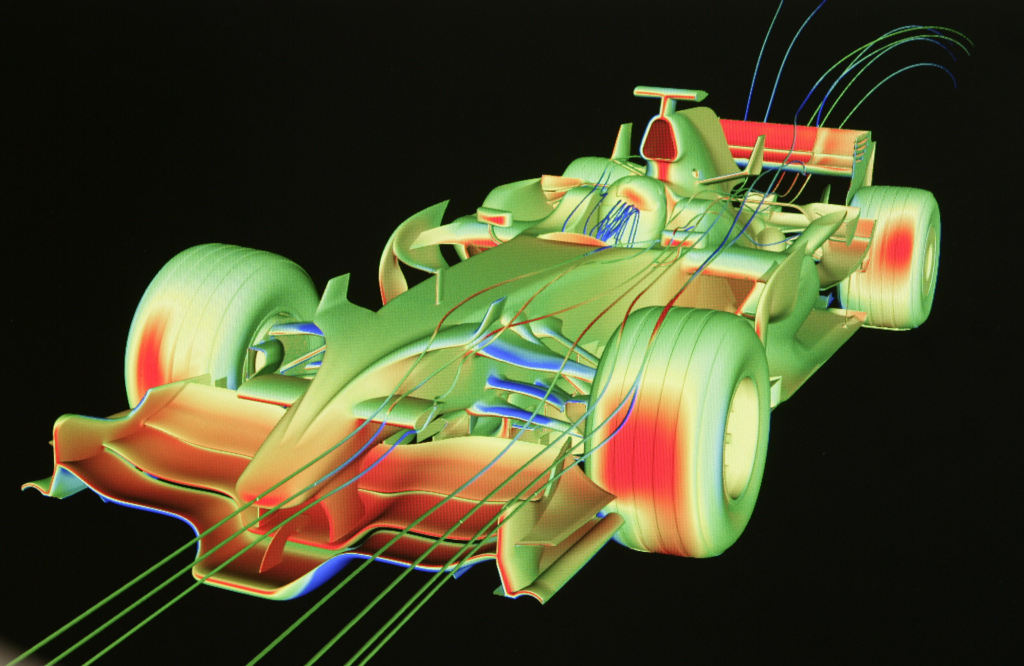
\includegraphics[width=\textwidth]{fmo1}
\end{center}
\end{columns}
\end{frame}

\section{Contenido general de la materia}

\begin{frame}{1. Propiedades de los fluidos}
\begin{exampleblock}{}
\begin{itemize}
\item Sistemas de unidades
\item Transformación de unidades
\item Definición de presión y esfuerzo de corte
\item Ley de viscosidad de Newton
\item Tipos de fluidos y tipos de flujo
\item Propiedades de los fluidos
\item Ecuación de estado de los gases y gases perfectos
\end{itemize}
\end{exampleblock}
\end{frame}

\begin{frame}{2. Est\'atica de los fluidos}
\vspace{-0.9cm}
\begin{columns}
\column{0.6\textwidth}
\begin{exampleblock}{}
\begin{itemize}
\small
\item Fluidos en reposo, escala de medida de la presión y de temperatura
\item Ecuación fundamental de la estática de los fluidos, fluido incompresible, fluido compresible, principio de Pascal
\item Aparatos medidores de presión
\item Fuerzas sobre cuerpos sumergidos: superficies planas, superficies curvas, principios de flotación
\item Equilibrio relativo de fluidos en movimiento
\item Aceleración lineal uniforme, rotación uniforme alrededor de un eje vertical
\item \alert{Laboratorios: Aparatos medidores de presión, Ensayos de flotación, Propiedades de los fluidos (banco de estática), Aparato de Reynolds}
\end{itemize}
\end{exampleblock}
\column{0.4\textwidth}
\begin{center}
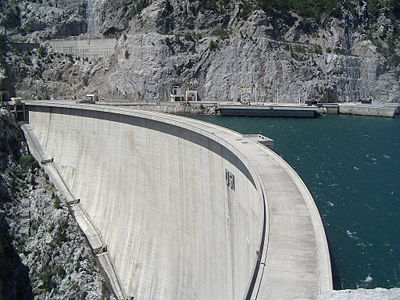
\includegraphics[width=\textwidth]{fme}
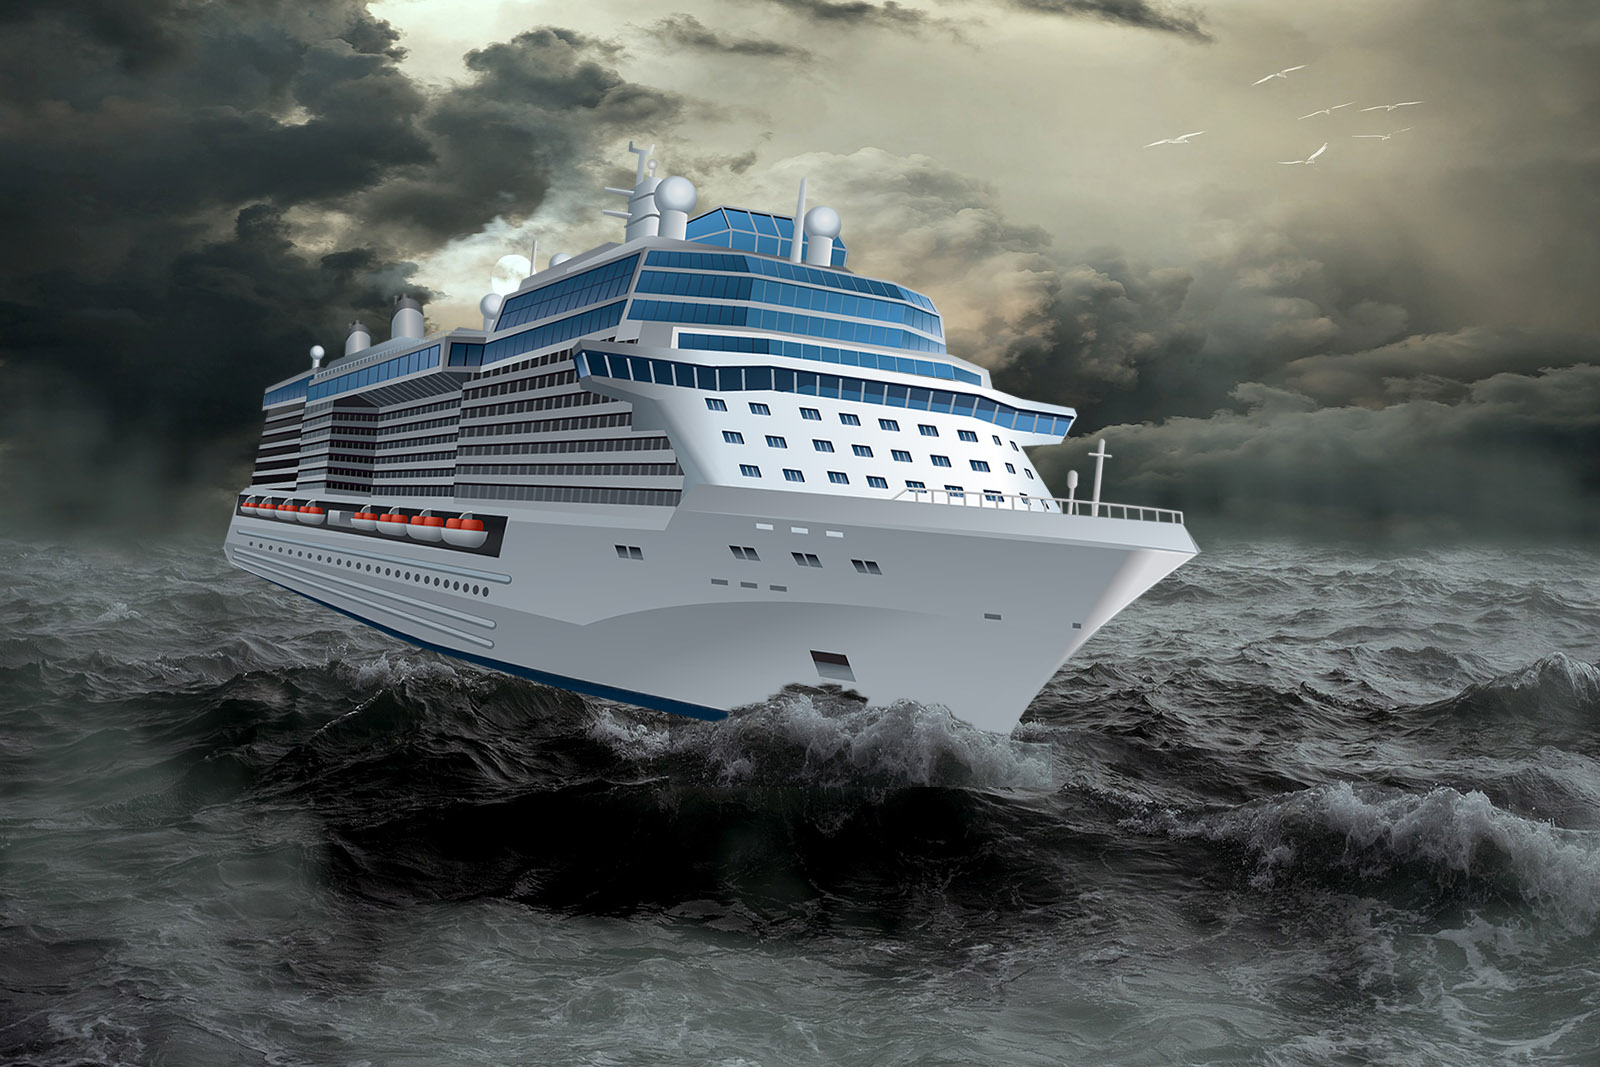
\includegraphics[width=\textwidth]{fme1}
\end{center}
\end{columns}
\end{frame}

\begin{frame}{3. Cinem\'atica de los fluidos}
\vspace{-0.9cm}
\begin{columns}
\column{0.6\textwidth}
\begin{exampleblock}{}
\begin{itemize}
\item Generalidades, propiedades cinemáticas del flujo
\item Métodos para describir el movimiento de un fluido: método de Lagrange y método de Euler
\item Flujo volumétrico y flujo másico, línea de corriente y clasificación de los flujos
\item Teorema de Transporte de Reynolds, ecuación de continuidad para un volumen de control, continuidad en un punto
\item Flujo potencial y función de corriente, relación entre flujo potencial y función de corriente
%\item \alert{Laboratorio: Hele-Shaw}
\end{itemize}
\end{exampleblock}
\column{0.4\textwidth}
\begin{center}
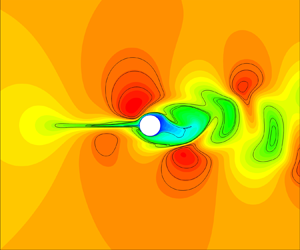
\includegraphics[width=\textwidth]{fmk}
\end{center}
\end{columns}
\end{frame}

\begin{frame}{4. Din\'amica de los fluidos}
\vspace{-1.2cm}
\begin{columns}
\column{0.6\textwidth}
\begin{exampleblock}{}
\begin{itemize}
\footnotesize
\item Ecuación de energía para flujos incompresibles y significado físico
\item Concepto de línea de energía, línea de gradiente hidráulico y potencia hidráulica
\item Aplicaciones de la ecuación de energía a sistemas de conducción: tuberías, canales, sistemas de bombeo, sistemas de generación hidroeléctrica
\item Medidores de caudal: orificios, tubo Pitot, tubo Venturi, medidor de codo
\item Cantidad de movimiento: cantidad de movimiento lineal aplicado a: estructuras hidráulicas como compuertas, vertederos, salto hidráulico, accesorios en tuberías, álabes fijos y móviles. 
\item Cantidad de movimiento angular.
\scriptsize
%\item \alert{Laboratorios: Línea de energía y línea de gradiente hidráulico, Flujo compresible, Tubo Pitot, Aparatos medidores de caudal: orificio, tubo Venturi.}
\item \alert{Laboratorios: Conservaci\'on de la energ\'ia y de la Cantidad de Movimiento Lineal.}
\end{itemize}
\end{exampleblock}
\column{0.4\textwidth}
\begin{center}
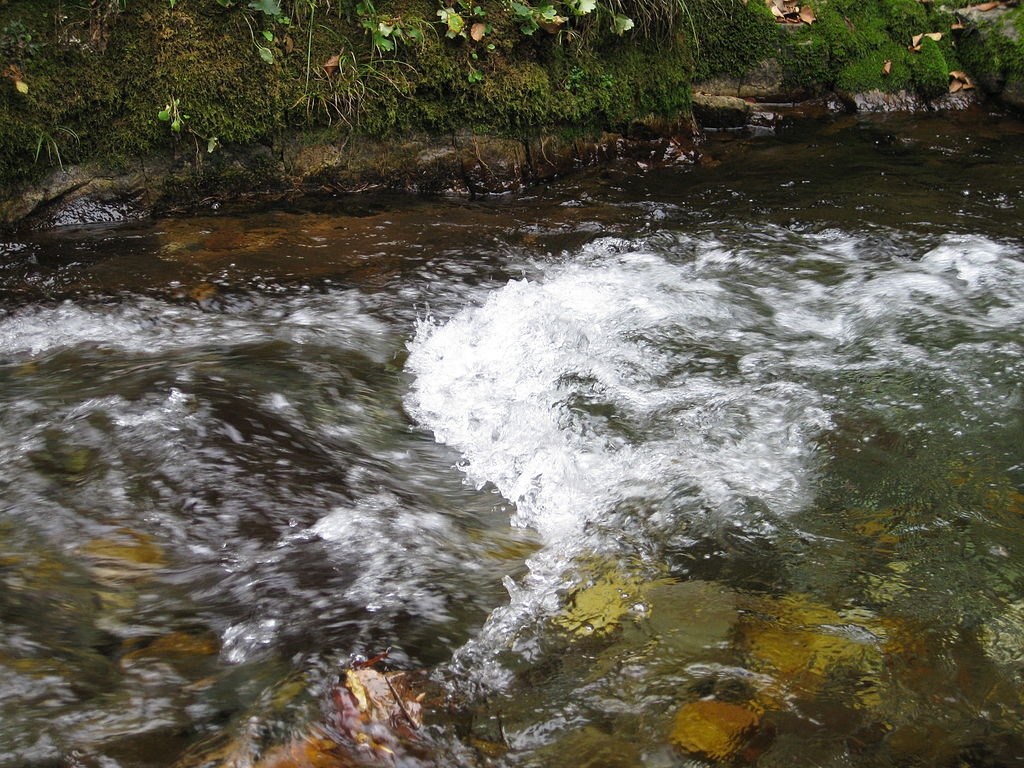
\includegraphics[width=\textwidth]{fmd}
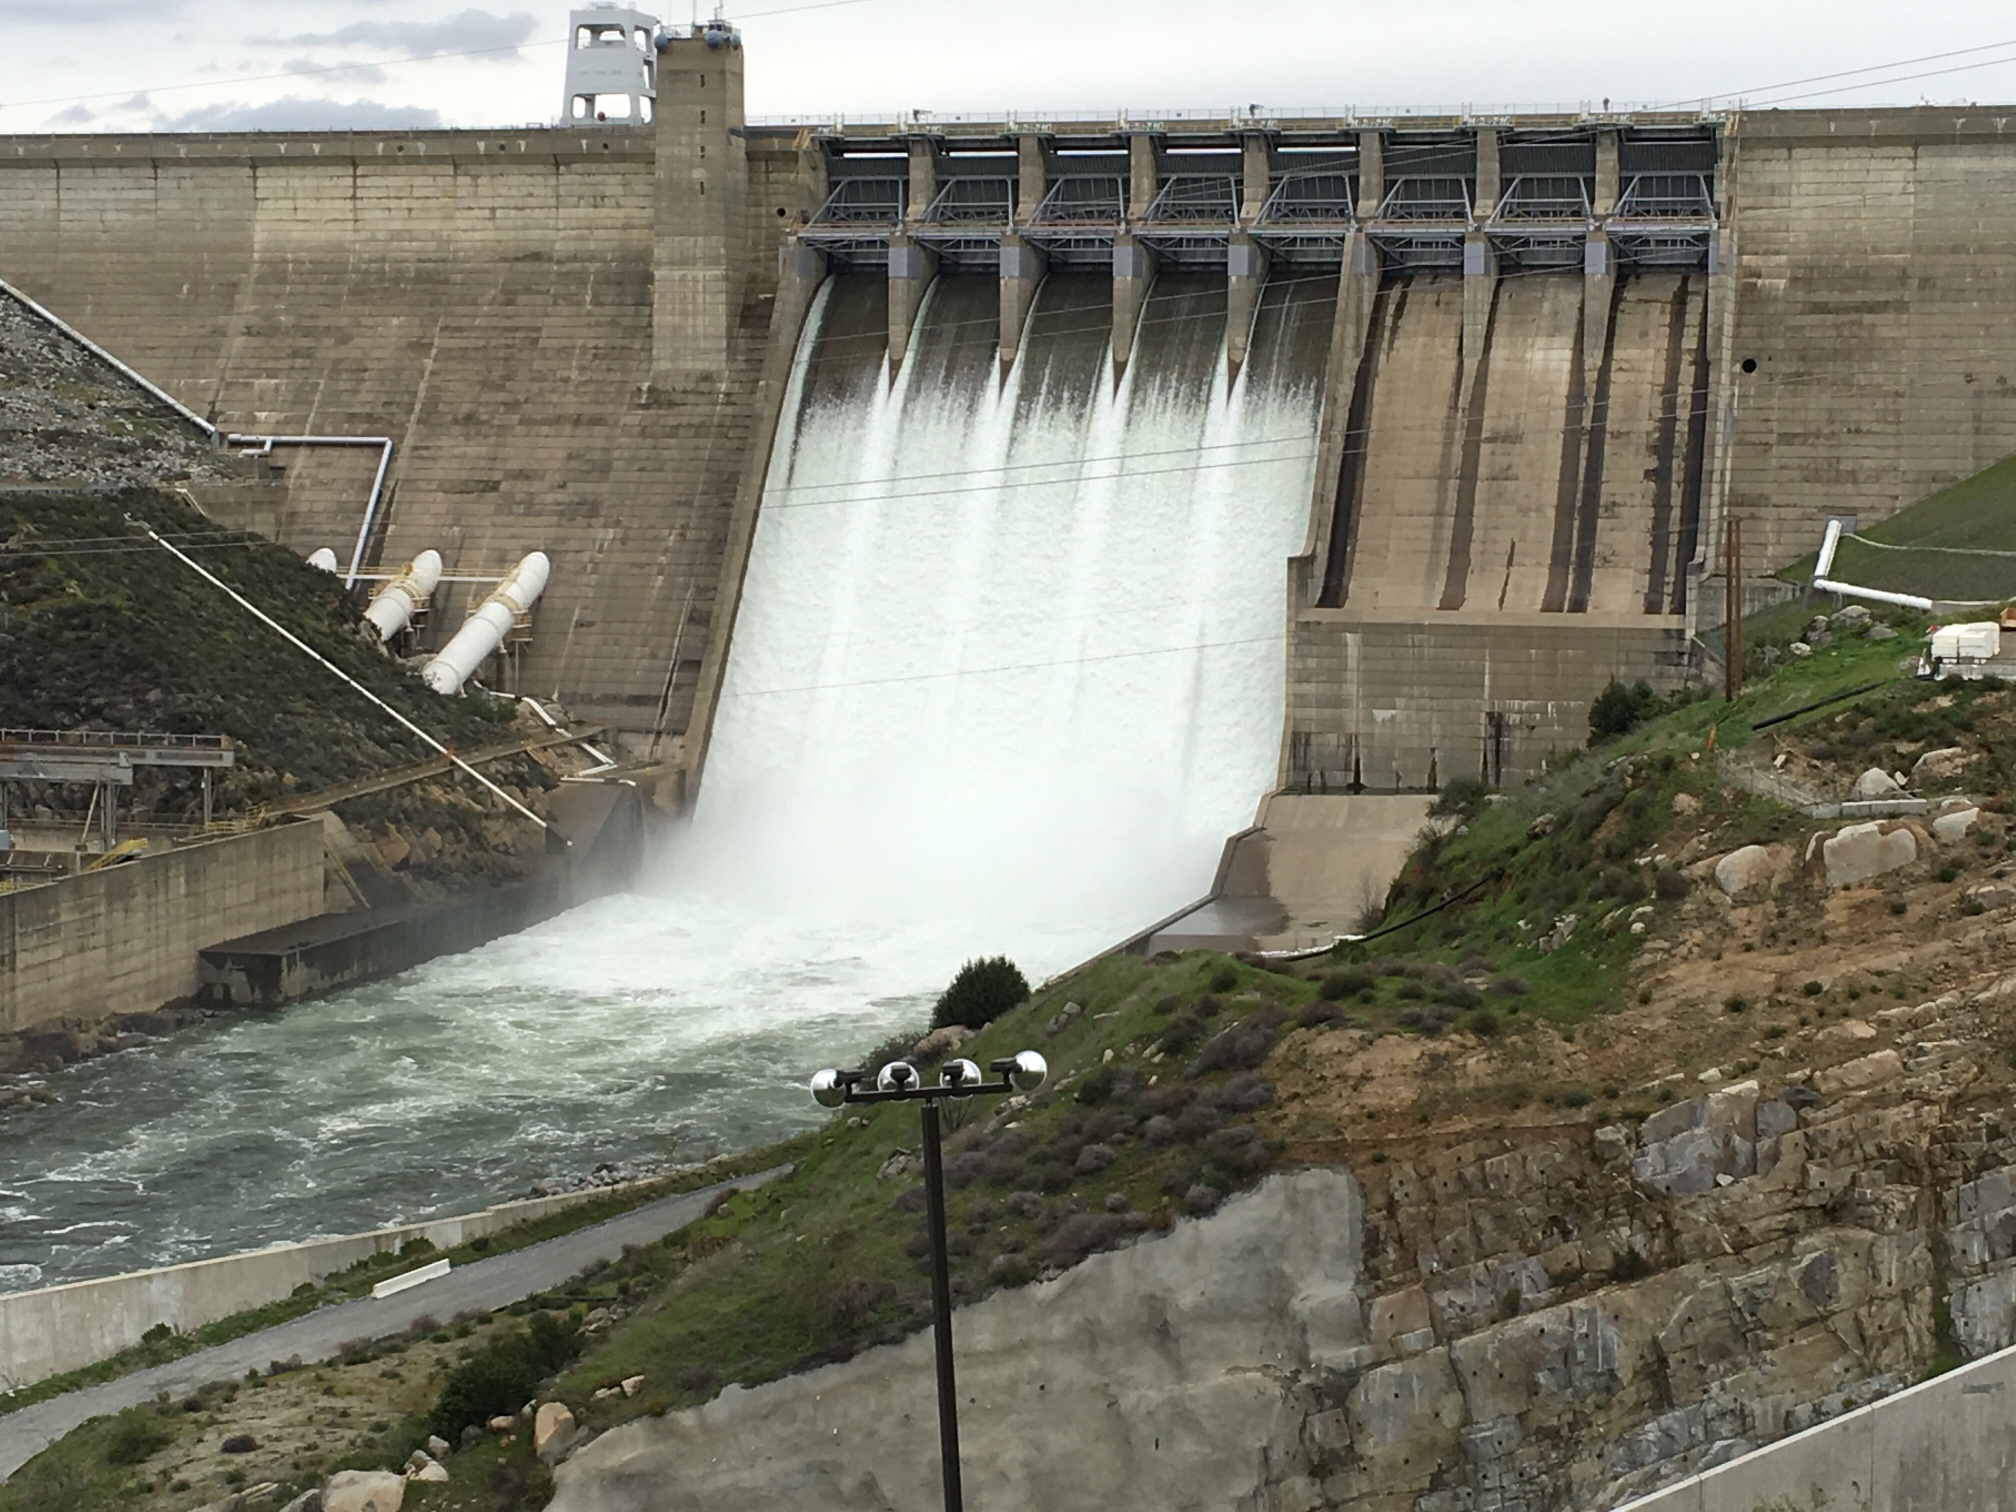
\includegraphics[width=\textwidth]{fmd1}
\end{center}
\end{columns}

\end{frame}

\begin{frame}{5. Analisis dimensional}
\begin{columns}
\column{0.5\textwidth}
\begin{exampleblock}{}
\begin{itemize}
\item Ecuación dimensionalmente homogénea
\item Parámetros adimensionales relevantes en mecánica de fluidos
\item Obtención de ecuaciones y teorema pi de Buckingham
\item Determinación de los grupos adimensionales y leyes de semejanza
\item Clasificación de los modelos físicos y aplicaciones
\end{itemize}
\end{exampleblock}
\column{0.5\textwidth}
\begin{center}
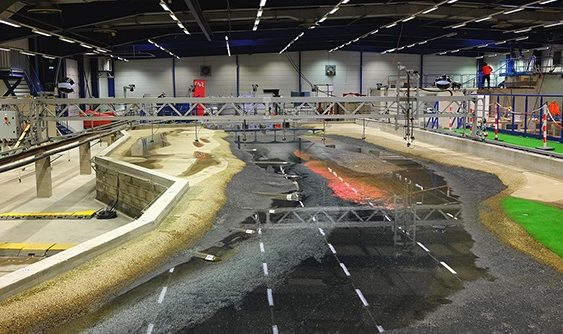
\includegraphics[width=\textwidth]{dimana}
\end{center}
\end{columns}
\end{frame}

\section{Evaluaci\'on del curso}
\begin{frame}{Evaluaci\'on del curso}
\centering
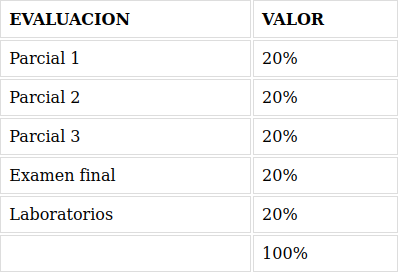
\includegraphics[width=9cm]{eval}
\end{frame}

\section{Referencias}
\begin{frame}{Referencias}
\begin{block}{Recomendadas}
\begin{enumerate}
\item \textbf{Çengel, Y. A., \& Cimbala, J. M. (2010). Fluid Mechanics: Fundamentals and Applications, McGraw-Hill Higher Education.}
\item \textbf{Duarte, C. A. (2017). Mecánica de fluidos e hidráulica, Universidad Nacional de Colombia, Facultad de Ingeniería,Departamento de Ingeniería Civil y Agrícola.}
\item \textbf{White, F. (2015). Fluid Mechanics, McGraw-Hill Higher Education.}
\end{enumerate}
\end{block}
\end{frame}

\begin{frame}{Referencias}
\begin{block}{Otros}
\begin{enumerate}
\small
\item Franzini, J. B., \& Finnemore, E. J. (1997). Fluid Mechanics with Engineering Applications: McGraw-Hill.
\item Liu, C. (2013). Schaum’s Outline of Fluid Mechanics and Hydraulics, 4th Edition: McGraw-Hill Education.
\item Mott, R. L. (2006). Applied Fluid Mechanics: Pearson Prentice Hall.
\item Potter, M. C., Wiggert, D. C., \& Ramadan, B. H. (2016). Mechanics of Fluids, SI Edition: Cengage Learning.
\item Pritchard, P. J. (2010). Fox and McDonald's Introduction to Fluid Mechanics, 8th Edition: John Wiley \& Sons.
\item Roberson, J. A., \& Crowe, C. T. (1999). Engineering Fluid Mechanics: Jaico Publishing House.
\item Shames, I. H. (1992). Mechanics of Fluids: McGraw-Hill.
\item Sotelo, G. (1974). Hidráulica general: fundamentos: Limusa.
\item Street, R. L., Watters, G. Z., \& Vennard, J. K. (1995). Elementary Fluid Mechanics: Wiley.
\item Streeter, V. L., \& Wylie, E. B. (1979). Fluid mechanics: McGraw-Hill.
\end{enumerate}
\end{block}
\end{frame}

%\begin{frame} [allowframebreaks]\frametitle{References}
               
%        \bibliographystyle{apalike}
%        \bibliography{bibfile}
%\end{frame}

\end{document}

